%% Преамбула TeX-файла

%[utf8x]
% 1. Стиль и язык
\documentclass[12pt]{G7-32} % Стиль (по умолчанию будет 14pt)
\usepackage[T2A]{fontenc}
\usepackage[russian]{babel}
%\nobibliography{rpz}
%\usepackage{bibentry}
%\setcitestyle{authoryear, open={((},close={))}}

% Остальные стандартные настройки убраны в preamble.inc.tex.
\sloppy

% Настройки стиля ГОСТ 7-32
% Для начала определяем, хотим мы или нет, чтобы рисунки и таблицы нумеровались в пределах раздела, или нам нужна сквозная нумерация.
\EqInChapter % формулы будут нумероваться в пределах раздела
\TableInChapter % таблицы будут нумероваться в пределах раздела
\PicInChapter % рисунки будут нумероваться в пределах раздела

% Добавляем гипертекстовое оглавление в PDF
\usepackage[
bookmarks=true, colorlinks=true, unicode=true,
urlcolor=black,linkcolor=black, anchorcolor=black,
citecolor=black, menucolor=black, filecolor=black,
]{hyperref}

% Изменение начертания шрифта --- после чего выглядит таймсоподобно.
% apt-get install scalable-cyrfonts-tex

%\usepackage[numbers,sort&compress]{natbib}


\IfFileExists{cyrtimes.sty}
    {
        \usepackage{cyrtimespatched}
    }
    {
        % А если Times нету, то будет CM...
    }

\usepackage{graphicx}   % Пакет для включения рисунков

% С такими оно полями оно работает по-умолчанию:
% \RequirePackage[left=20mm,right=10mm,top=20mm,bottom=20mm,headsep=0pt]{geometry}
% Если вас тошнит от поля в 10мм --- увеличивайте до 20-ти, ну и про переплёт не забывайте:
\geometry{right=20mm}
\geometry{left=30mm}


% Пакет Tikz %%%/// МНЕ НЕ НУЖНО, это для черчения фигур
%\usepackage{tikz}
%\usetikzlibrary{arrows,positioning,shadows}

% Произвольная нумерация списков.
%\usepackage{enumerate} %%%/// МНЕ НЕ НУЖНО, это для custom наименований пунктов списка

% ячейки в несколько строчек
\usepackage{multirow}

% itemize внутри tabular
\usepackage{paralist,array}


% Настройки листингов.
% 8 Листинги

\usepackage{listings}

% Значения по умолчанию
\lstset{
  basicstyle= \footnotesize,
  breakatwhitespace=true,% разрыв строк только на whitespacce
  breaklines=true,       % переносить длинные строки
%   captionpos=b,          % подписи снизу -- вроде не надо
  inputencoding=koi8-r,
  numbers=left,          % нумерация слева
  numberstyle=\footnotesize,
  showspaces=false,      % показывать пробелы подчеркиваниями -- идиотизм 70-х годов
  showstringspaces=false,
  showtabs=false,        % и табы тоже
  stepnumber=1,
  tabsize=4,              % кому нужны табы по 8 символов?
  frame=single
}

% Стиль для псевдокода: строчки обычно короткие, поэтому размер шрифта побольше
\lstdefinestyle{pseudocode}{
  basicstyle=\small,
  keywordstyle=\color{black}\bfseries\underbar,
  language=Pseudocode,
  numberstyle=\footnotesize,
  commentstyle=\footnotesize\it
}

% Стиль для обычного кода: маленький шрифт
\lstdefinestyle{realcode}{
  basicstyle=\scriptsize,
  numberstyle=\footnotesize
}

% Стиль для коротких кусков обычного кода: средний шрифт
\lstdefinestyle{simplecode}{
  basicstyle=\footnotesize,
  numberstyle=\footnotesize
}

% Стиль для BNF
\lstdefinestyle{grammar}{
  basicstyle=\footnotesize,
  numberstyle=\footnotesize,
  stringstyle=\bfseries\ttfamily,
  language=BNF
}

% Определим свой язык для написания псевдокодов на основе Python
\lstdefinelanguage[]{Pseudocode}[]{Python}{
  morekeywords={each,empty,wait,do},% ключевые слова добавлять сюда
  morecomment=[s]{\{}{\}},% комменты {а-ля Pascal} смотрятся нагляднее
  literate=% а сюда добавлять операторы, которые хотите отображать как мат. символы
    {->}{\ensuremath{$\rightarrow$}~}2%
    {<-}{\ensuremath{$\leftarrow$}~}2%
    {:=}{\ensuremath{$\leftarrow$}~}2%
    {<--}{\ensuremath{$\Longleftarrow$}~}2%
}[keywords,comments]

% Свой язык для задания грамматик в BNF
\lstdefinelanguage[]{BNF}[]{}{
  morekeywords={},
  morecomment=[s]{@}{@},
  morestring=[b]",%
  literate=%
    {->}{\ensuremath{$\rightarrow$}~}2%
    {*}{\ensuremath{$^*$}~}2%
    {+}{\ensuremath{$^+$}~}2%
    {|}{\ensuremath{$|$}~}2%
}[keywords,comments,strings]

% Подписи к листингам на русском языке.
\renewcommand\lstlistingname{\cyr\CYRL\cyri\cyrs\cyrt\cyri\cyrn\cyrg}
\renewcommand\lstlistlistingname{\cyr\CYRL\cyri\cyrs\cyrt\cyri\cyrn\cyrg\cyri}


% Полезные макросы листингов.
% Любимые команды
\newcommand{\Code}[1]{\textbf{#1}}


\begin{document}

\frontmatter % выключает нумерацию ВСЕГО; здесь начинаются ненумерованные главы: реферат, введение, глоссарий, сокращения и прочее.

% Команды \breakingbeforechapters и \nonbreakingbeforechapters
% управляют разрывом страницы перед главами.
% По-умолчанию страница разрывается.

% \nobreakingbeforechapters
% \breakingbeforechapters

%% Также можно использовать \Referat, как в оригинале
\begin{abstract}
тра-тата

\end{abstract}

%%% Local Variables: 
%%% mode: latex
%%% TeX-master: "rpz"
%%% End: 


%% $Id: diploma-title.tex 52 2009-06-04 09:46:14Z zyv $

\thispagestyle{empty}

\begin{center}

        \textsc{Федеральное агентство по образованию}\\[0.2cm]

        \textsc{Государственное образовательное учреждение высшего
профессионального образования \\ <<Иракский государственный университет
им.~Д.В.~Буша>>}\\[0.7cm]

        Арбузолитейный факультет\\[0.5cm]

        Специальность <<Фундаментальный исламизм и физическая
софистика>>\\[0.7cm]

        Кафедра общей демократии\\[0.7cm]

        \textsc{Дипломная работа}\\[0.7cm]

        \begin{large}
                \textsc{\textbf{Восстановление архитектуры разрушенных
городов по многобахчевым дынным полям методом всеобщего голосования}}
        \end{large}

\end{center}

\vspace{0.7cm}

\textit{<<К защите допущен>>:}

\begin{center}
        \begin{tabular}{ll}
                Зав. кафедрой общей демократии, \\
                профессор, д.ф.-м.н. &
                        \begin{tabular}{ll}
                                \underline{\phantom{Четкая подпись}} &
                                Иванов И.И.
                        \end{tabular}
        \\[0.7cm]
                Научный руководитель, \\
                профессор, в.н.с. ЁКЛ ЭМЭН,\\
                д.ф.-м.н. &
                        \begin{tabular}{ll}
                                \underline{\phantom{Четкая подпись}} &
                                Петров П.П.
                        \end{tabular}
        \\[0.7cm]
                Рецензент, \\
                зав. лаб. ЖЗ ИКЛ,\\
                д.ф.-м.н. &
                        \begin{tabular}{ll}
                                \underline{\phantom{Четкая подпись}} &
                                Сидоров С.С.
                        \end{tabular}
        \\[0.7cm]
                Консультант по технике\\
                безопасности, ассистент\\
                каф. софистики &
                        \begin{tabular}{ll}
                                \underline{\phantom{Четкая подпись}} &
                                Рейсфейдер Р.Р.
                        \end{tabular}
        \\[0.7cm]
        Дипломник &
                        \begin{tabular}{ll}
                                \underline{\phantom{Четкая подпись}} &
                                Ватманн В.В.
                        \end{tabular}
        \end{tabular}

        \vspace{1.5cm}

        г. Анкара, 2009

\end{center}
\tableofcontents

%%$tex

\Introduction

\textbf{Цель} данной работы -- литургико-исторический анализ особого чина пострижения в великую схиму женщин, известного также как \emph{пострижение черниц ангельского образа}, бытовавшего на Руси в XIV--XVII вв..

Для достижения поставленной цели необходимо:

\begin{itemize}
\tightlist
\item
  описать структуру и состав чина по его представлению у Н. Красносельцева и по оригинальным источникам
\item
  проанализировать особенности, отличающие чин от мужского пострига в великую схиму
\item
  проанализировать возможные предпосылки к формированию чина в чинопоследованиях крещения, хиротоний и поставления дев
\end{itemize}

\textbf{Актуальность} выбранной темы связана с тем, что последнее подробное описание чина сделано Н. Ф. Красносельцевым в 1889г., с тех пор стало известно больше источников, в т.ч. описан Дмитриевским Евхологий 1027г. №213, исследован и восстановлен в католической церкви чин поставления дев и т.д..
Также, настоящее время предъявляет всё больше вопросов как к христианскому пониманию иночества, так и к женскому служению в церкви.
Чин пострижения черниц ангельского образа позволяет исследовать как определённые, сохранившиеся в древнем чине антропологические воззрения на иночество и служение, так и их гендерное преломление.

\textbf{Степень изученности и источники}.
В русских требниках от XV и до сер. XVII вв. совместно с чином пострижения в великую схиму мужчин, можно найти особый чин для постригающихся женщин, «чин пострижения черниц ангельского образа».
Он встречается в рукописях, хранящихся в Соловецкой библиотеке, библиотеке Троице-Сергиевой Лавры и в более поздних печатных Московский потребниках: Филаретовском (1625г.), Иноческом (1639г.), Иосифофском (1651г.).
В ходе книжной справы 1640-60-х гг., чин исчезает, т.к. отсутствует в греческих книгах, по которым проводилась справа.
В настоящее время для мужского и женского пострига предназначен один чин.

Женский чин пострижения в великую схиму был найден вновь и описан Н.В. Красносельцевым как «чин пострижения черниц»\cite[С.~134–169]{@krasnoseltcev.uprazdnenniye.1889} в ходе исследования рукописей Соловецкой библиотеки.
Несмотря на исчезновение из требников, чин как и монашеская традиция вызывали большой интерес в XIX веке, о чём может свидетельствовать его описание в реалистическом романе «На горах» П. Мельникова-Печерского\footnote{Роман «На горах» написан в 1874-75 гг., что ненамного, но опережает выход книги Н. Красносельцева с описанием чина -- в 1889 г.. Вероятно, он провёл самостоятельные исследования, а также мог получить консультацию от бывшего старообрядца, уставщика Рогожского кладбища Василий Борисов, ставший прототипом Василия Борисыча в его романах. \textit{За этот факт автор работы благодарит Боченкова В., автора книги о Мельникове–Печерском.}}, с подробным и правильным приведением начальных строк особых стихир и антифонов чина, а также верно описанной структурой.

Наиболее раннее изложение этого чина было найдено проф. А. Дмитриевским в Евхологии 1027г. Парижской Национальной (Coislin) библиотеки №213\cite[С.~1035–1042]{dmitriyevskiy.opisaniye.1901}.
В Русской Церкви наиболее ранний источник -- славяно-русский Требник XIVв. Московской Троице-Сергиевой лавры №229, ЛЛ. 29--35, где он появляется под названием «Служба скымихя на пострижениiе черницам».
Согласно гипотезе Н. Пальмова, он мог попасть в русскую церковь благодаря юго-славянскому влиянию на русское богослужение XIVв.\cite[С.~14]{palmov.postrijeniye.1914}, чему дополнительное свидетельство -- аналогичный чин с похожим названием «Служба на пострижениiе черноризици» в юго-славянском Требнике Имп. СПБ. Публ. библ. №21 из собрания А. Ф. Гильфердинга, ЛЛ. 37--51.




\mainmatter % это включает нумерацию глав и секций в документе ниже

%\chapter{Чин, его структура и составные элементы}\label{ux433ux43bux430ux432ux430-1-ux447ux438ux43d-ux435ux433ux43e-ux441ux442ux440ux443ux43aux442ux443ux440ux430-ux438-ux441ux43eux441ux442ux430ux432ux43dux44bux435-ux44dux43bux435ux43cux435ux43dux442ux44b}

\section*{Общие замечания}\label{ux43eux431ux449ux438ux435-ux437ux430ux43cux435ux447ux430ux43dux438ux44f}

Чин пострижения черниц ангельского образа во многом повторяет мужской постриг в великую схиму, но с некоторыми заметными изменениями.
Во-первых, служба предваряется обрядом омовения ног постригающейся, который совершает игуменья.
Во-вторых, многие песнопения изменены по сравнению с мужским постригом.

В данной работе, как и в источниках, слова «как в мужском чине пострига» отсылают к постригу мужчин в великую схиму в ту же эпоху (XIV--XVIIвв.).
Существующий в настоящее время единый чин великой схимы отличается.

\section*{Омовение ног}\label{ux43eux43cux43eux432ux435ux43dux438ux435-ux43dux43eux433}

Начинается обряд после утрени, когда в келью желающей принять постриг приходят инокини.
Песнопения в этом месте специально подобраны к женскому чину.
Что интересно, они непосредственно обращены к постригающейся.
После первой стихиры, в чине появляется священник (здесь непонятно, вышли ли из кельи к нему, или вошёл он вместе с сёстрами).

Структура последования (выделены действия):

\begin{itemize}
\tightlist
\item
  \textbf{инокини приходят в келью к постригаемой}
\item
  инокини поют стихиру: «Послушай Христа, что вопиет дево, крест вземше иго мое на раме»
\item
  священник творит обычное начало
\item
  Псалом 50
\item
  Канон великой схимы
\item
  \textbf{игуменья за руку ведёт постригаемую} в притвор церкви, \textbf{монахини со свечами следуют за ними и поют} стихиру: «Последуимъ сестры благому владыце, увядимъ мiрскихъ похотей» и богородичен: «Грешныхъ молитвы прiемлюще скорбящихъ въздыханiе»
\item
  поют три антифона, третий («Союзомъ любви связуеми апостоли») взят из чина омовения ног в Великий Четверг
\item
  ектенья
\item
  две молитвы из чина омовения ног
\item
  Евангелие от Иоанна, в ходе чтения \textbf{игуменья препоясывается «понявою» и умывает ноги желающей принять пострижение и отирает их «лентiемъ»}
\item
  во время омовения ног, трижды поют стихиру: «Умый нозе честная мати и обуй мя сапогомъ целомудрiя, да не пришедъ врагъ обрящетъ пяты моя нагы и запнетъ стопы моя» и богородичен: «Имуще тя, Богородице, упованiе»
\item
  дочитывается Евангелие (вероятно, имеется ввиду зачало от слов «Когда же Он умыл их ноги и взял одежду Свою и возлёг снова, Он сказал им: знаете ли, что Я сделал вам? (Ин 13:12))
\item
  поётся тропарь «Господа глашаете мя и учителя» со стихом «Окропиши мя иссопомъ», \textbf{игуменья и монахини кропят «на лица своя отъ воды умыванiя»}
\end{itemize}

\section*{Литургия слова и пострижение}\label{ux43bux438ux442ux443ux440ux433ux438ux44f-ux441ux43bux43eux432ux430-ux438-ux43fux43eux441ux442ux440ux438ux436ux435ux43dux438ux435}

После омовения ног в притворе, игменья, постригаемая и сёстры входят в церковь.
По входу в церковь, начинается литургия с чином пострижения в великую схиму и особыми антифонами, тематически подобранными к женскому постригу.
По ходу пения антифонов, постригаемая движется к алтарю, с тремя остановками: в начале (притворе), у амвона и перед царскими вратами.

Постриг продолжается в два этапа: сперва постригает священник, а затем сёстры -- в дьяконнике или на паперти.
Так же происходило и в мужском чине.
Иногда между постригами было целование постригае(мой/ого).
Иногда второй этап пострига совершался при участии небольшого числа братьев (сестёр), а именно восприемников.

\begin{itemize}
\tightlist
\item
  \textbf{игуменья, постригаемая и сёстры входят в церковь с пением} тропаря «Къ тебе утреннюемъ милосердому умывше нозе» и богородичен: «Избави насъ от бедъ нашихъ мати Христа Бога»
\item
  великая ектенья
\item
  1-й антифон: «Хотех слезами омыти моихъ греховъ, Господи, рукописанiе\ldots{}»
\item
  \textbf{постригаемая подходит к амвону}
\item
  2-й антифон: «Где есть мирская краота, где есть временныхъ мечтанiе\ldots{}»
\item
  \textbf{постригаемая подходит к царским вратам}
\item
  3-й антифон: «Господи отверзи двери чертога рабе твоей\ldots{}»
\item
  «Придите, поклонимся»
\item
  на «Придите, поклонимся», \textbf{постригаемая простирается ниц у царских врат} до конца богородична
\item
  стихира «Прiидите ко мне вси труждающiеся» и богородичен «Иже тебе ради Богоотецъ пророкъ Давидъ»
\item
  следуют \textbf{вопросы священника и ответы постригаемой}, те же, что и в мужском постриге, начиная с: «Что прiиде, сестро, припадая къ святому жертвеннику?»
\item
  \textbf{пострижение}
\item
  \textbf{сёстры вводят постригаемую в диаконник или на паперть и постригают}, воспевая целиком 17-ю кафизму («Блаженны непорочные»)
\item
  в это время читаются Апостол и Евангелие, что и в мужском постриге
\end{itemize}

\section*{Литургия верных и облачение}\label{ux43bux438ux442ux443ux440ux433ux438ux44f-ux432ux435ux440ux43dux44bux445-ux438-ux43eux431ux43bux430ux447ux435ux43dux438ux435}

После пострига, сёстры вновь ведут новопостриженную в церковь.
Следует её второе приближение к алтарю с тремя новыми антифонами и остановками в тех же местах.
В этот раз по приближении к царским вратам, её вводят в алтарь и начинается облачение.

\begin{itemize}
\tightlist
\item
  \textbf{новопостриженную сестру вводят в церковь} «въ конечней ризе\footnote{Имеется ввиду срачица.}, неопоясану, непокровенну, необувенну»
\item
  3 антифона «Евангельского гласа вскоре повеленiе исполнила еси»
\item
  во время пения антифонов \textbf{новопостриженная приближается к алтарю и к третьему встаёт у царских врат}
\item
  \textbf{новопостриженная входит в алтарь}
\item
  \textbf{священник облачает её в великосхимнические одежды}, комментируя каждый предмет облачения. В это время сёстры поют стихиры, что и в мужском пострижении
\item
  молитвы священника: Господи Боже нашъ введи рабу твою» и «Господи Боже нашъ, верныхъ въ обетованiи»
\item
  стихиры «Да возрадуется душа моя о Господе», «Сорадйтеся ми о Христе сестры» и др.
\item
  \textbf{целование Евангелия и новопостриженной}: дьякон встаёт в царских вратах, держа Евангелие вне врат. Новопостриженная целует Евангелие и встаёт рядом с дьяконом. Игуменья и сёстры по очереди целуют Евангелие, а затем новопостриженную и трижды поют стихиру на 1-й глас: «Разумеимъ сестры таинства силу» и богородичен «Радуйся Богородице, дево, радуйся похвало»
\item
  литургия далее завершается как обычно
\end{itemize}

\section*{Трапеза и третье введение в церковь}\label{ux442ux440ux430ux43fux435ux437ux430-ux438-ux442ux440ux435ux442ux44cux435-ux432ux432ux435ux434ux435ux43dux438ux435-ux432-ux446ux435ux440ux43aux43eux432ux44c}

В завершение пострижения игуменья, новопостриженная и сёстры покидали храм для совершения трапезы.
После трапезы, игуменья вновь вводила за руку новопостриженную в церковь, где та оставалась 7 дней до молитвы на снятие кукуля.
На 8-й день над ней читается та же молитва на снятие кукуля, что и в мужском постриге.

\begin{itemize}
\tightlist
\item
  после отпуста литургии \textbf{сёстры с новопостриженной выходят из церкви на трапезу с пением} тех же стихир, что и в мужском постриге
\item
  по окончанию трапезы поются стихиры «Аще внешняго совлечеся одеянiя» и «Премудрый Павелъ невестоводитель бываетъ на небесехъ тайно принося мир обрученiе Христово»
\item
  \textbf{игуменья за руку вводит новопостриженную в церковь в третий раз}
\item
  в это время сёстры поют стихиры «Господи, Господи, призри съ небесе и виждь» и богородичен «Свеще неугасимая»
\item
  в церкви поются несколько песнопений, специально выбранных для женского пострижения, последнее из которых «Чистъ ест бракъ и нескверненъ, о дево, неугасиму свещу соблюдай всегда»
\item
  по окончанию пения \textbf{сёстры расходятся по кельям, а новопостриженная остаётся в церкви}
\end{itemize}

\include{21-Ch.1.2TEST}
%\chapter{Особенности действий и песнопений в чине}\label{ux433ux43bux430ux432ux430-2-ux43eux441ux43eux431ux435ux43dux43dux43eux441ux442ux438-ux434ux435ux439ux441ux442ux432ux438ux439-ux438-ux43fux435ux441ux43dux43eux43fux435ux43dux438ux439-ux432-ux447ux438ux43dux435}

\section*{Омовение ног}\label{ux43eux43cux43eux432ux435ux43dux438ux435-ux43dux43eux433-1}

Обряд омовения ног является вступлением к постригу.
В мужских чинах ничего подобного не встречается.
По структуре и содержанию молитв, чтений, песнопений, действий, он почти полностью повторяет омовение ног в кафедральных соборах в Великий Четверг.
Обряд в этот день совершался также и в монастырях, где как и в исследуемом чине, его совершал игумен(ья)\cite[С.~149]{krasnoseltcev.uprazdnenniye.1889}.

По поводу соединения чина с постригом, Красносельцев предполагает причину в приурочении чинов поставления дев к определённым праздникам (Пасха, апостолов Петра и Павла, Богоявления), подобно крещениям.
Об этом пишет и св. Амвросий Медиоланский в Exhortatio virginatis: «пришёл день Пасхи: во всём мире совершаются таинства крещения, возлагаются покрывала на священных дев».
Великий четверг же оказывался днём, к которому приурочивали множество священнодействий, в т.ч. совершаемых епископом: освящение мира, воссоединение кающихся, общее елеосвящение.
Вероятно, и освящение дев, которое тоже мог творить только епископ, совершалось в этот день.
Так, соединённые в записях, чины могли слиться, когда были забыты изначальные смыслы их нахождения рядом\cite[С.~150]{krasnoseltcev.uprazdnenniye.1889}.

Омовению ног предшествуют не встречающееся в чине Великого Четверга песнопения.
По входу в келью желающей принять постриг, сёстры поют стихиру:

\textit{Послушай Христа, что вопиетъ, о дево. крестъ вземши, иго мое на раму, иди отвержися земныхъ. да не привлечетъ тебе страсть. ни пища чревная тя лишитъ, истиннаго живота. внемли, утвержай страшное обещание. где пасетъ, где пребываетъ. егоже любитъ душа моя.
}

Потом, с зажжёнными свечами, следуя за игуменьей и постригаемой в притвор:

\textit{Последуемъ сестры благому владыце, увядимъ мирския похоти. бежимъ лестьца мира, и миродержителя. будемъ чисти и совершени, почтемъ образъ, устыдимся звания. преложимъ житие. что творимся сами смирени, высоцы бывше. что в видимыхъ пребываемъ. темъ каяждо насъ себе плодъ принесетъ Христови, по данней ей благодати. давсякими мерами добродетелей, тамо сущая славы обители наследуемъ.}

Небольшие изменения касаются объекта прошений на ектенье и в молитвах, который из «нас» превращается в «её».
Так, в молитве «Боже преблагий, неприступный божествоъ, иже во зраце рабий служителя образъ восприемый», появляется «греховныя скверны омы ти рабы своея, \emph{имрк.}, сподоби прикосновениемъ воды сея. да чиста душею же и теломъ бывши, благоугодно ти послужит\ldots{}».

\section*{Антифоны}\label{ux430ux43dux442ux438ux444ux43eux43dux44b}

Как уже было сказано, песнопения в чине значительно отличаются по тематики от используемых в мужском постриге на Руси в это время.
Последние объединены темой покаяния в образе возвращения блудного сына\cite[С.~144–145]{krasnoseltcev.uprazdnenniye.1889}.
Женские же песнопения связаны с темами возрастания в добродетели и духовном бодрствовании в образах обручения с Женихом и ожидания Его подобно разумным девам с горящими светильниками:

Первый антифон -- стихира покаянная в неделю вечера на 4-й глас, также поющаяся в неделю о самарянке.
В ней есть образ и покаяния, и невесты: «коль возлюблена села твоя Господи силъ\ldots{} единъ человеколюбецъ Богъ нашъ тя ныне приемлет дево, того всею душею возлюбивши, потому покажи чистое житие. угоди успешно зовящи\ldots{}».
Постригаемая сравнивается с возлюбленной и призывается хранить верность этой любви (ещё пока не браку).
Здесь есть и дерзновенное прошение возлюбленной: «приими мя ходящую во следъ тебе, краснаго жениха моего. не попусти врагу хвалитися мною\ldots{}».

Второй антифон развивает эти образы, становясь как бы иллюстрацией библейской Песни Песней: «Распни уды христолюбивая. умертви страсти воздержаниемъ, и к жениху си теци и взови. где пасеши женише. где живеши рцы ми. яко тебе возлюбивши притекох. на рамо крестъ твой вземши. да вниду в чертогъ свещу носящи, ико дева чистая\ldots{}».
Здесь постригаемая сравнивается с взывающей и ищущей жениха возлюбленной.
К этому яркому, порывистому образу примыкают крест, горящая свеча, чистота, а позже мученица Фекла, риза нетления, Богородица -- образы верности и испытанности.

К третьему антифону постригаемая стоит перед царскими вратами, и в это время поётся: «Господи, отверзи двери чертога рабе твоей, верою припадающи\ldots{}».
Так, образ ищущей чертога жениха в песнопениях дополняется движением к чертогу-алтарю в ходе службы.
В антифоне есть прошения: «сподоби ю всесилне, святаго твоего звания, и спричти ю паствы твоея, Иисусе мой. хотяй спасти всех нас, и отверзи двери правды\ldots{} Отверзи двери правды, вшед в ня\ldots{} Господи, оружие ми подай же на ратоборца. верою и надеждою и любовию укрепи мя всесилне нань яко человеколюбец. побеждьши его съкрушу и поеру, хотяй всех нас спасти».
Здесь о постригаемой молятся как о воине, выходящем на битву с лукавым.

\section*{Шествие под пение антифонов}\label{ux434ux432ux438ux436ux435ux43dux438ux435-ux432ux43e-ux432ux440ux435ux43cux44f-ux430ux43dux442ux438ux444ux43eux43dux43eux432}

Дважды втечение литургии постригаемая движется от притвора к алтарю под пение антифонов.
В разных источниках, её движение заканчивается у царских врат либо уже в алтаре, сперва для пострига, а во второй раз -- для облачения.
Первое движение происходит под антифоны на литургии слова, второе -- на литургии верных.

В этом шествии можно увидеть остатки динамики кафедрального станционного богослужения, когда подобное движение от притвора к амвону и затем к алтарю (а клиром -- в алтарь) совершалось всей паствой.
Там вход в храм совершался на месте нынешнего «малого входа», а к амвону приступали во время пения Трисвятого для слушания Писания и проповеди.
К алтарю приступали на «великом входе» литургии верных.

В чинах постригов эта логика разрушена и остался лишь динамический импульс шествия.
К сожалению, он оторван от смысла собственно литургии и происходит параллельно.
Особенно это заметно в том, что во время чтения постригаемая и сёстры вовсе отсутствуют.
Они в дьяконнике либо в притворе совершают вторую, «братскую» часть пострига и возвращаются лишь с началом литургии верных.

Возможно, этот разрыв богослужебной логики произошёл в связи с многослойностью самого чина пострига, вобравшего, по-видимому, в себя содержание малого и великого постригов, а впоследствие ещё подвергнутого попыткам «свернуть» чин обратно в один из постригов.

\section*{Первый вход в алтарь: постриг}\label{ux432ux445ux43eux434-ux432-ux430ux43bux442ux430ux440ux44c-ux43fux43eux441ux442ux440ux438ux433}

Вход в алтарь тем более интересен, что в настоящее время ни в мужском, ни в женском постриге в великую схиму, постригаемый не вводится в алтарь, если только это не дьякон или священник.

Также интересно, что постриг имеет два этапа: пострижение священником и пострижение сёстрами (по некоторым версиям -- воспреемниками) в дьяконнике или на паперти.
Последнее весьма адекватно чину, т.к. монахиня принимается не только игуменьей, но и сестричеством.

В настоящее время пострижение в великую схиму, подобно пострижению в мантию, не имеет второго этапа пострига.
Ектенья на постриге переходит прямо в ектенью на облачении, а постриг рукой священника -- в облачение тут же, у царских врат.
После того следует обычное завершение чина пострига в великую схиму, а затем -- обычное завершение литургии.
Подобный сокращённый чин великой схимы встречается в Евхологии Афоно--Дионисиатской библ. №450 и предназначен для тех, кто уже прошёл чин малого пострига.

С одной стороны, это выявляет «составную» структуру чина великой схимы, которая, вероятно, сохранилась со времён чина изложенного в Евхологии Барберини св. Марка, где также соединены малая и великая схима.
Таким образом, можно увидеть изначальную внутреннюю логику: постриг соответствовал литургии слова, а облачение -- литургии верных.

Согласно Пальмову, сокращение в Евхологии №450 избавило чин от лишнего, повторяющегося обряда пострига, сохранив лишь обряд облачения, т.к. мантийный монах уже пострижен и его основное отличие -- облачение.
Нельзя не заметить, однако, что сокращение чина выполнено неудачно, с перемещением обряда облачения, логически соответствующего литургии верных, в литургию слова.

Современное же состояние чинов оказывается вовсе неудачным: из малой схимы исчезла вторая часть пострига, а великая схима переместилась целиком в литургию слова.
Таким образом, пострижение братьями (сёстрами) вовсе исчезло из современного чина, а облачение потеряло свой торжественный символизм, связанный с литургией верных.

\section*{Второй вход в алтарь: облачение}\label{ux432ux445ux43eux434-ux432-ux430ux43bux442ux430ux440ux44c-ux43eux431ux43bux430ux447ux435ux43dux438ux435}

По возвращению в церковь после чтения Писания, постригаемая вновь продвигается под пение антифонов к царским вратам.
Далее следует облачение.
По разным источникам оно совершается либо «близ» (видимо, имеется ввиду близ царских врат), либо сказано «вшедше же ей в олтарь».
Последнее встречается в ряд русских источников более раннего происхождения (Требники №998 (XVв.), №1004 (XIVв.)).
Второй из этих требников, при этом, описывает облачение в чине мужского пострига «близ» (Л.139), а женское -- в алтаре (Л.126).
Вероятно, раз разделившись, эти два чина развивались самостоятельно.

Пальмов пишет, что согласно правильному переводу места облачения «τὸ βλῆμα» в греческих Евхологиях, «облачение в великосхимнические одежды необходимо представлять происходящим в алтаре у св. престола»\cite[С.~147]{palmov.postrijeniye.1914}.

%\chapter{Реконструкция истоков чина}

\section*{Крещение}

В «оглашении» в чине великой схимы есть слова «О новаго звания! О дара тайны! Второе крещение приемлеши днесь, брате, богатствомъ человеколюбца Бога даровъ, и отъ греховъ твоихъ очищаешися, и сынъ света бываеши», а в молитве «Сый Владыко Вседержителю, вышний Царю славы» -- «Сопричти его избраннымъ Твоимъ, да будетъ Твой сосудъ избранный, сынъ и наследникъ Царствия Твоего\ldots{}».
Эти и другие черты сближают чин пострига в великую схиму с крещением.

Согласно Н. Пальмову\cite{palmov.postrijeniye.1914}, эти элементы появились в современном типе чина благодаря редакции преп. Феодора Студита.
В X--XIвв. чин уже имел такой вид, согласно Евхологию Московского Румянцевского Музея № 474 и Евхологию 1027г. Парижской Национальной (Coislin) библиотеки.
В более ранней редакции, в Евхологии Барберини св. Марка эти элементы отсутствуют и чин имеет другой облик.

Впрочем, эти элементы присутствуют и в мужском постриге.
Разница в тематизме песнопений: в женском чине образ сочетания со Христом выступает гораздо явственнее.

\section*{Чины хиротоний}\label{ux447ux438ux43dux44b-ux445ux438ux440ux43eux442ux43eux43dux438ux439}

Облачение в алтаре более всего напоминает чины поставления на служение.

Введение в алтарь встречается уже в наиболее раннем из известных нам чинов пострижения в Евхологии Барберини\cite[С.~210–216]{barberini.evhologiy.2011}.
Этот чин, один из древнейших известных чинов монашеского пострига, состоит из двух частей: малого и великого пострига.
В ходе малого пострига, «отрекающийся входит в святилище и приклоняется перед святым жертвенником», что бывает также в чинах рукоположения, в т.ч. диаконисс\footnote{Правда, диакониссы при рукоположении лишь приклоняли главу. Диакон вставал на одно колено, а пресвитер -- на оба.}.
О рукоположении диаконисс в алтаре пишет Неселовский\cite[С.~72]{neselovskiy.4ini.1906}, ссылаясь на Матфея Властаря, основного свидетеля по этому вопросу.
Далее, одна из молитв древнего чина имеет слова: «Господи Боже истины, именем твоим \textbf{возлагаю руку мою на твоего раба} \emph{имярек}\ldots{} чтобы \textbf{служил всегда твоей благости}, поклоняясь и восхваляя твоё имя святое, прославляя тебя во все дни его жизни\ldots{}».

В чине пострижения черниц ангельского образа осталось простирание перед царскими вратами (и алтарём) перед постригом, после чего священник поднимал постригащуюся за руку.
Также, присутствует облачение в алтаре.
Антифоны сохранили прошения о духовных дарованиях.

Облачение завершается перед анафорой, и в некоторых источниках сообщается, что новому схимонах(у/ине) давалась свеча, с которой он(а) участвовал(а) в великом входе со свечой\cite{palmov.postrijeniye.1914} (вероятно, предстоя перед вратами как делают сейчас алтарники).

Хотя маловероятно, что непосредственно хиротония диаконисс повлиял на женский чин великой схимы, но в целом родство с чинами поставления на служение прослеживается.
Присутствует даже своеобразное литургическое «служение» (свеча).

\section*{Чин поставления дев}\label{ux447ux438ux43d-ux43fux43eux441ux442ux430ux432ux43bux435ux43dux438ux44f-ux434ux435ux432}

Красносельцев упоминает возможные истоки образности песнопений чина и более ранних молитв из Евхология Барберини\footnote{Имеются ввиду шесть молитв №258--263 «на пострижение монахинь»\cite[С.~176–178]{barberini.evhologiy.2011}} в чинах поставления дев и вдовиц церковных\cite[С.~145–146]{krasnoseltcev.uprazdnenniye.1889}.
В обоих случаях основным является образ обручения с небесным женихом и ожидания его с горящим светильником.

Девы и вдовицы не рукополагались, о чём сказано в Апостольском предании, среди упоминания других церковных чинов (Trad. Ap. 12), однако в IVв. на Западе формируется velatio\footnote{В дальнейшем чин дев упоминается в произведениях св. отцов на Востоке до Vв.. Вероятно, в дальнейшем он был вытеснен женским монашеством и диакониссами, разделившими его функции. На Западе сохранялся особый чин посвящения в дев до XIIIв., который был возрождён в 1970г. в результате II Ватиканского Собора.} -- особый чин посвящения дев через возложение плата им на голову и чтение молитв\cite{pravenc.devy.20}.
В 6-м правиле Карфагенского поместного собора предписывается «освящение дев» не творить пресвитеру и многие комментаторы, в т.ч. Красносельцев трактуют это как возможность совершать чин только епископу.

Согласно Красносельцеву, обряд посвящения в девы состоял из принесения обета девства, «увещания епископа», возложения на голову посвящаемой покрывала.
Это покрывало -- flammeum virginale.
Согласно античной традиции, при вступлении в брак, на голову женщины надевался плат, называемый flammeum (или velum).
Эта деталь обряда бракосочетания вошла в обряд посвящения в девы, став в нём вещественной символикой брака.\\
Девы назывались «невестами Христовыми» начиная с Тертуллиана.

Как минимум до запрета 45-м правилом Шестого вселенского собора, существовал обычай перед пострижением одевать женщину в дорогие костюмы и украшения, словно невесту, и в таком виде приводить в храм.

В чине поставления дев, представленном в сакраментарии Геласия (ок. 750г.), присутствуют молитвы, которые с незначительными изменениями вошли в состав современного посвящения в девы, восстановленного католической церковью после II Ватиканского собора.
В этих молитвах также присутствует мотив Жениха-Христа: «They give themselves wholly to Christ, the Son of the ever-virgin Mary, and the heavenly Bridegroom of those who in hist honor dedicate themselves to lasting virginity\footnote{Здесь и далее молитвы из чина поставления дев цитируются по новому католическому чину, на английском языке.}» и даётся образ рождения от Духа: «Your children are born, not of human birth, nor of man's desire, but of your Spirit».
Но, значительно больше внимания уделяется образу девства: «They place in your hands their resolve to live in chastity\ldots{} Among your many gifts you give to some the grace of virginity\ldots{} Those who choose chastity have looked upon the face of Christ, its origin and inspiration\ldots{} in his honor dedicate themselves to lasting virginity\ldots{}» -- четыре и даже более упоминания девственности втечение одной молитвы!
И Христос также описан как образец и вдохновение для целибата.

Так, в чине поставления дев основное внимание оказывается на личном подвиге девства, а не на браке со Христом, как в постриге черниц ангельского образа.
В обоих чинах присутствуют прошения на укрепление и защиту от искушений, но в чине дев отсутствует образ брани духовной и ожидания со свечой в руках Жениха.
Последний образ может быть особенно важной отличительной чертой русского чина, потому как сообщает ему эсхатологическое измерение и дополняет яркую тему влюблённости духовной трезвостью взыскующей нетленного царства.

Помимо этих отличий, есть и важное сходство, касающееся вне-литургического аспекта обоих чинов.\\
Одна из задач чина дев, согласно свт. Амвросию Медиоланскому, -- укрепление для преодоления сопротивления христианству в семье: «та, которая победила дом, победила век» (Ambros. Mediol. De virginib. 1. 12. 64).
А согласно 140 правилу Карфагенского Собора, -- и для укрепления «в опасности угрожающей целомудрию девы, когда есть подозрение или о любителе сильном, или о каком либо похитителе».

Итак, выделяются две тематические линии: 1) бракосочетание с Женихом-Христом и 2) укрепление уз семьи духовной для преодоления сопротивления как собственной плоти, так и семьи по плоти.
Вероятно, обе они оказывались актуальными и на Руси в среде женского иночества XIV--XVIIвв..

XIX век как время особого раскола между церковным и светским обществом, вдвойне привлекал внимание к этим темам.
Первая привлекала своим мистицизмом уставшую от просвещенческого рационализма интеллигенцию, вторая оказывалась актуальна для верующих женщин в среде светского небрежного, а иногда и агрессивного отношения к церкви.
Здесь можно вспомнить такие произведения как роман «Дворянское гнездо» Тургенева, где героиня против воли семьи уходит в монастырь, картину Нестерова «На горах» и многие другие его картины, связанные с образами монашества и великой схимы.
Наконец, в романе Мельникова-Печерского «На горах» даётся довольно выпуклый образ на эту же тему: читатель видит чин глазами купца, страстно влюблённого в монахиню и надеющегося похитить её из монастыря.
Когда он признаёт в постригающейся ту самую, кого чаял похитить, его мечты рассыпаются.



%
\nocite{virgin.catholic.1970}
\nocite{trebnik.1884}
\nocite{taft.statyi.2011}
\nocite{lotmanl.melnikov.1956}
\nocite{pravenc.velatio.20}

\backmatter %% Здесь заканчивается нумерованная часть документа и начинаются ссылки и
            %% заключение

%%$tex

\Conclusion % заключение к отчёту

Чин пострижения черниц ангельского образа -- яркий, самобытный и особенно интересный как сохранивший и древние особенности монашеских чинов, и, вероятно, ещё более древнюю литургическую образность обручения с Женихом.
Он вызывает и исследовательский интерес как совмещающий в себе множество элементов различных богослужений: чин омовения ног, чин малой схимы, чин великой схимы, антифонное шествие кафедрального последования литургии.
Он интересен и сам по себе как ярко образный, динамичный, особенно благодаря двум антифонным шествиям и входам-выходам.

Чину присуща определённая поэзия, вероятно не только сохранённая, но и доосмысленная и обогащённая особенностями как русской, так и женской души.
Образы, знаки, символы в чине поэтически переплетаются: свеча в руке и Богородица как свеча, образы совлечения ветхой одежды и движение в одной сорочке к облачению в алтаре, чертог Жениха искомый возлюбленной и вход в алтарь, где на престоле -- Св. Дары.

С другой стороны, уже в своём первоначальном виде чин являет проблемы, характерные для смешения, расширения в «слабых местах»\cite{taft.rastut.2009} и последующего урезания важных смысловых моментов.
Так, главная бросающаяся в глаза проблема -- смысловая разделённость, параллельность совершающегося пострига и литургии, при их внешнем динамическом объединении.
Другая проблема, которую чин унаследовал от предшественников -- запутанность соединения чинов малой и великой схимы.
Спор о необходимости слияния ступеней монашеского пострига в одну держится с эпохи преп. Феодора Студита и до наших дней, а попытки то разделить, то объединить чины, не пошли им на пользу.


%%% Local Variables: 
%%% mode: latex
%%% TeX-master: "rpz"
%%% End: 



% % Список литературы при помощи BibTeX
% Юзать так:
%
% pdflatex rpz
% bibtex rpz
% pdflatex rpz

\bibliographystyle{gost780u}
\bibliography{aspiro_1.0}

%%% Local Variables: 
%%% mode: latex
%%% TeX-master: "rpz"
%%% End: 


\appendix   % Тут идут приложения

%\chapter{Некоторые из молитв «образа» (258--263), изложенные в Евхологии Барберини св. Марка}\label{ux43dux435ux43aux43eux442ux43eux440ux44bux435-ux438ux437-ux448ux435ux441ux442ux438-ux43cux43eux43bux438ux442ux432-ux43e-ux43cux43eux43dux430ux445ux438ux43dux435-258263-ux438ux437ux43bux43eux436ux435ux43dux43dux44bux435-ux432-ux435ux432ux445ux43eux43bux43eux433ux438ux438-ux431ux430ux440ux431ux435ux440ux438ux43dux438-ux441ux432.-ux43cux430ux440ux43aux430}

Здесь изложены четыре из шести молитв Евхология Барберини св. Марка\cite[С.219–222]{barberini.evhologiy.2011}, наиболее схожие с текстами антифонов чина пострижения черниц ангельского образа и, вероятно, послужившие основой для них.

\textbf{{[}258{]}} Молитва о принимающей образ монашеский.\\
Господи Боже наш, так возлюбивший девственность, что назначил матерью твоего домостроительства, сам, Владыкa всяческих, прими твою рабыню \emph{имярек}, восхотевшую оставить эту мирскую и преходящую славу и созерцать твою благость, и удостой ее посещения твоего Духа Святого, даруй ей воздержание и всяческую скромность чтобы, живя угодно тебе, как сияние благоразумия несла светильник, непрестанно исполняясь елеем своих дел, навстречу тебe, жениху небесному. Ибо благословенно и прославлено (твое имя) достойное хвалы.

\textbf{{[}259{]}} Вторая молитва о монахине.\\
Боже благ, Отец девственности и возделыватель добродетельной жизни, сохрани эту рабыню твою в красоте избранной, облачи ее сиянием святости и одеждой целомудрия, чтобы заботилась о Господнем, как угодить Владыке, чтобы была святой в телe, в душе и в духе, и, сопричисляясь к сонму разумных дев и неся светильник благочестия, удостоилась войти в небесные чертоги жизни вечной. Во Христе Иисусе Господе нашем, с которым ты благословен, со пресвятым и благим и животворящим.

\textbf{{[}260{]}} Третья молитва образа.
Господи Боже нашa, призывающий праведников к святости и грешников к оправданию, и обращающихся быть помилованными, сам, Господи человеколюбец, прими обращение твоей рабыни \emph{имярек}, и по благости прости ее, припадающую перед твоим милосердием в исповедании своих грехов. Искупи ее от всякого греха, да воссияет над всяким нечистым помышлением, очисти ее от всякой скверны плоти и духа и укрепи в исполнении заповедей твоих, сняв с нее суету мирскую и отрезав ей волосы в подражание твоей первомученице Фекле; сделай ее сопричисленной к верным и разумным девам, чтобы в чистоте души и тела принoся добрый плод и возрастая в добрых делах, стала наследницей царства небесного. Во Христе Иисусе Господe нашем с которым ты благословен, с пресвятым и благим.

\textbf{{[}262{]}} Пятая молитва образа.
Свят, Свят, обитающий в святыхa, хотящий, чтобы все люди спас- лись и пришли в познание истиныb, так возлюбивший род челове- ческий что вселился и пребывал в немc чтобы он был храмoм твоей славы страшной и бессмертной, ты сказал: если кто хочет идти за мною, да отвергнется от себя, и возьмeт крест свой, и последует за мноюd, сам, Владыка человеколюбец, благоволи к отречению твоей рабыни имярек, наложи на нее иго твое благое и бремя твое легкоеe, сохрани цельными ее Дух, душу и телоf, облачи ее в одежду первуюg духовную и нетленную, одень ее броней верыh и всеоружием Духа Святогоi, препоясай ее чистотой, святостью, целомудриемj, чтобы укрепившись твоей силой против козней дьявольскихk, подвизаться подвигом добрым, совершить твой путь, сохранить твою веруl и получить венец праведностиm, который ты обещал любящим тебяn и соблюдающим твои заповеди. Ибо подобает тебе всякая славаo, честь и поклонение.

%\chapter{Источники XIV–XVвв. о введении женщин в алтарь на постриге или облачении}
\label{cha:appendix1}

\begin{figure}[h]
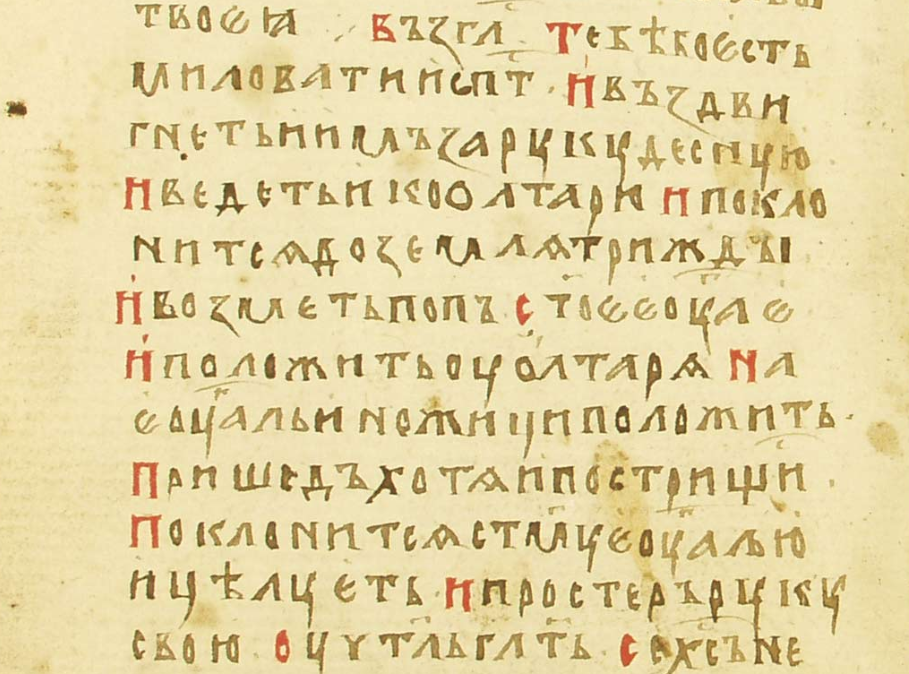
\includegraphics[width=1\linewidth]{14c._altar_hair}
\caption{Введение в алтарь на постриг. Требник XIVв. №998}
\label{14c._altar_hair}
\end{figure}

%%% Local Variables: 
%%% mode: latex
%%% TeX-master: "rpz"
%%% End: 

%\chapter{Проповеди язычникам}
\label{cha:appendix2}

\subsection*{Проповедь ап Павла в Листрах (Деян 14:8-18}
8 И некий муж в Листрах, не владевший ногами, сидел; хромой от чрева матери своей, он никогда не ходил.

9 Он слышал, как говорил Павел, который, устремив на него взор и увидев, что он имеет веру, чтобы быть спасенным,

10 сказал громким голосом: встань на ноги твои прямо. И он вскочил и стал ходить.

11 Народ же, увидев, что сделал Павел, возвысил свой голос, говоря по-ликаонски: боги в образе человеческом сошли к нам.

12 И называли они Варнаву Зевсом, а Павла Гермесом, так как он держал речь.

13 И жрец Зевса, стоящего перед городом, доставив к воротам быков и венки, хотел с народом принести жертву.

14 Но апостолы Варнава и Павел, услышав, разорвали одежды свои и с криком бросились в толпу,

15 говоря: мужи, что это вы делаете? И мы – подобные вам люди, благовествующие вам, чтобы вы от этих суетных богов обратились к Богу живому, Который сотворил небо и землю, и море и всё, что в них,

16 Который в прошедших поколениях позволил всем народам ходить своими путями,

17 хотя и не переставал свидетельствовать о Себе, творя добро, подавая вам с неба дожди и времена плодоносные, исполняя пищею и радостью сердца ваши.

18 И говоря это, они едва успокоили народ, чтобы не приносили им жертвы.

\subsection*{Проповедь ап Павла в Ареопаге (Деян 17:16-34)}
16 И пока Павел ожидал их в Афинах, дух его в нем возмущался, видя, что город полон идолов.

17 Итак, он рассуждал в синагоге с Иудеями и чтущими Бога, и на площади каждый день со случайными встречными.

18 А кое-кто и из эпикурейских и стоических философов встречался с ним, и некоторые говорили: что хочет сказать этот пустослов? А другие: кажется, это проповедник чужих богов (потому что он благовествовал Иисуса и воскресение).

19 И взяв его, привели в Ареопаг и говорили: можем ли мы узнать, что это за новое учение, проповедуемое тобой?

20 Ибо странное что-то вкладываешь ты в наши уши. Вот мы и хотим узнать, что это может быть?

21 Афиняне же все и живущие у них чужестранцы ничем другим не заполняли свои досуги, как тем, чтобы говорить или слушать что-нибудь новое.

22 И Павел, став посредине Ареопага, сказал: мужи Афиняне, по всему вижу, что вы особенно богобоязненны.

23 Ибо, проходя и осматривая ваши святыни, я нашел и жертвенник, на котором было написано: "неведомому богу". Итак, что вы, не зная, чтите, я возвещаю это вам.

24 Бог, сотворивший мир и всё, что в нём, Он, Господь неба и земли, не в рукотворенных храмах обитает,

25 и не руками человеческими воздается Ему служение, как имеющему в чем-либо нужду: Он Сам дарует всем жизнь и дыхание и всё.

26 И произвёл Он от одного весь род человеческий: обитать по всему лицу земли, предуставив сроки и пределы их обитанию;

27 искать Бога, не коснутся ли они Его и не найдут ли, хотя и не далеко Он от каждого из нас.

28 Ибо в Нем мы живем и движемся и существуем, как и некоторые из ваших поэтов сказали: "Ведь мы Его и род".

29 Итак, будучи родом Божиим, мы не должны думать, что Божество подобно золоту, или серебру, или камню, носящим печать искусства и мысли человеческой,

30 Поэтому, оставив без внимания времена неведения, Бог теперь возвещает людям, всем и всюду, чтобы они каялись,

31 ибо Он определил день, когда будет судить вселенную по праведности, чрез Мужа, Которого Он поставил, дав удостоверение всем, воскресив Его из мертвых.

32 Услышав же о воскресении мертвых, одни насмехались, другие сказали: мы послушаем тебя об этом еще раз.

33 Так Павел вышел из среды их.

34 Но некоторые люди, примкнув к нему, уверовали: между ними и Дионисий Ареопагит и женщина, по имени Дамарь, и другие с ними.

\subsection*{Проповедь ап Павла прокуратору Феликсу (Деян 24:10-26)}
10 И ответил Павел, когда правитель сделал ему знак говорить: зная, что ты с давних лет судишь этот народ, я с легким сердцем буду защищать мое дело,

11 так как ты можешь узнать, что – не более двенадцати дней, как я пришел для поклонения в Иерусалим.

12 И не нашли меня ни в храме с кем-либо спорящим или вызывающим волнение народа, ни в синагогах, ни в городе,

13 и не могут доказать тебе того, в чем теперь обвиняют меня.

14 Но в том я признаюсь тебе, что на Пути, который они называют ересью, я, действительно, служу Богу отцов наших, веруя всему, что согласно с Законом и что написано у Пророков,

15 надежду имея на Бога, которую и сами они разделяют, – что будет воскресение и праведных и неправедных.

16 Потому я и сам стараюсь всегда иметь непорочную совесть пред Богом и людьми.

17 Через несколько лет я прибыл с целью передать милостыни народу моему и приношения.

18 При этом нашли меня очистившимся в храме, не с толпой и не с шумом,

19 нашли же какие-то Иудеи из Асии, которым надлежало бы быть здесь у тебя и обвинять, если бы у них было что против меня.

20 Или пусть они сами скажут, какое нашли они преступление, когда я предстал пред синедрионом,

21 кроме одного этого слова, которое я возгласил, стоя между ними: "за воскресение мертвых вы меня судите сегодня".

22 Но Феликс, имея более точные сведения о Пути, отослал их для дополнительного расследования, сказав: когда придет трибун Лисий, я рассмотрю ваше дело;

23 и дал распоряжение сотнику держать его под стражей, но давать ему некоторые послабления, и не препятствовать никому из близких его служить ему.

24 Несколько дней спустя, Феликс, прибыв с Друзиллой, женой своей, Иудеянкой, послал за Павлом и слушал его о вере во Христа Иисуса.

25 Но так как он говорил о праведности и обладании собой и о будущем суде, то Феликс, придя в страх, ответил: пока иди, а при случае я тебя вызову к себе.

26 В то же время он и надеялся, что Павел даст ему денег. Потому-то, часто за ним посылая, он и беседовал с ним.

\subsection*{Проповедь ап Павла перед царём Агриппой (Деян 26:1-31)}
1 И сказал Агриппа Павлу: тебе разрешается говорить за себя. Тогда Павел, протянув руку, начал свою защитительную речь:

2 во всём, в чем обвиняют меня Иудеи, царь Агриппа, я почитаю себя счастливым защищаться сегодня перед тобой,

3 потому особенно, что ты знаток всех обычаев и спорных мнений Иудеев. Поэтому прошу выслушать меня с долготерпением.

4 Жизнь мою от юности, протекавшую с самого начала среди народа моего в Иерусалиме, ведают все Иудеи,

5 зная обо мне издавна, если есть у них желание свидетельствовать – что жил я фарисеем, по строжайшему направлению в нашей вере.

6 И теперь я стою перед судом за надежду на обещание, бывшее от Бога отцам нашим,

7 исполнения которого надеются достичь наши двенадцать колен, усердно служа Богу день и ночь. За эту надежду, царь, и обвиняют меня Иудеи.

8 Почему у вас считается невероятным, что Бог воздвигает мертвых?

9 Ведь я и сам думал, что против имени Иисуса Назорея надо мне многое сделать.

10 Это я и делал в Иерусалиме, и многих из святых я заключил в тюрьмы, получив власть от первосвященников, и когда их убивали, подавал свой голос против них;

11 и по всем синагогам, многократно наказывая их, принуждал к хуле и, в чрезмерной против них ярости, преследовал их даже и в чужих городах.

12 В этих условиях, отправляясь в Дамаск с полномочиями и поручением от первосвященников,

13 я в полдень на дороге увидел, царь, свет с неба, сильнее солнечного блеска, осиявший меня и шедших со мной.

14 И когда все мы упали на землю, я услышал голос, говорящий мне на еврейском языке: "Саул, Саул, что ты меня гонишь? Трудно тебе идти против рожна".

15 Я сказал: "Кто Ты, Господи?" Господь сказал: "Я Иисус, Которого ты гонишь.

16 Но встань и стань на ноги твои, ибо Я для того явился тебе, чтобы поставить тебя служителем и свидетелем Моим, как ты Меня видел, и как Я явлюсь тебе,

17 избавляя тебя от народа и от язычников, к которым Я посылаю тебя,

18 открыть им глаза, чтобы обратились они от тьмы к свету и от власти сатаны к Богу, и чтобы получили они отпущение грехов и удел вместе с освященными, по вере в Меня".

19 Поэтому, царь Агриппа, я не оказал непослушания небесному видению,

20 но сперва находящимся в Дамаске и Иерусалиме, и по всей стране Иудейской, и язычникам возвещал, чтобы они каялись и обращались к Богу, творя дела, достойные покаяния.

21 За это Иудеи, задержав меня в храме, пытались расправиться со мной.

22 Итак, с помощью, которая приходит от Бога, я устоял до сего дня, свидетельствуя малому и великому, не говоря ничего, кроме того, о чем Пророки сказали и Моисей, что должно тому быть:

23 Христу – пострадать и, воскресши первым из мертвых, свет возвещать народу и язычникам.

24 Когда он так защищался, Фест громким голосом говорит: ты безумствуешь, Павел! Большая ученость доводит тебя до безумия.

25 А Павел говорит: я не безумствую, превосходнейший Фест, но возглашаю слова истины и здравого смысла.

26 Ибо знает об этом царь, которому я и говорю с дерзновением. Ведь я не верю, чтобы сокрыто было от него что-либо из этого; ибо не в углу это было совершено.

27 Веришь ли, царь Агриппа, Пророкам? Знаю, что веришь.

28 Но Агриппа Павлу: еще немного, и ты будешь убеждать меня сделаться христианином.

29 А Павел: молил бы я Бога, чтобы мало ли, много ли, не только ты, но и все слушающие меня сегодня, сделались такими же как и я, кроме этих уз.

30 И встал царь и правитель и Вереника и сидевшие с ними,

31 и удалившись, говорили между собой, что ничего достойного смерти или уз человек этот не делает.

%%% Local Variables: 
%%% mode: latex
%%% TeX-master: "rpz"
%%% End: 



\end{document}

%%% Local Variables:
%%% mode: latex
%%% TeX-master: t
%%% End:
